\documentclass[11pt,a4paper]{article}
\usepackage[margin=2.2cm,headheight=15pt,headsep=16pt]{geometry}
\usepackage{fontspec}
\IfFontExistsTF{Times New Roman}{\setmainfont{Times New Roman}}{\setmainfont{TeX Gyre Termes}}
\IfFontExistsTF{Arial}{\setsansfont{Arial}}{\setsansfont{TeX Gyre Heros}}
\usepackage{amsmath,amssymb}
\usepackage{graphicx,booktabs,tabularx,array}
\usepackage{xcolor}
\usepackage{caption}
\usepackage{placeins}
\usepackage{fancyhdr}
\usepackage{titlesec}
\usepackage[numbers,sort&compress]{natbib}
\usepackage{xurl}
\usepackage{hyperref}
\definecolor{navy}{HTML}{183A50}
\hypersetup{colorlinks=true,linkcolor=navy,citecolor=navy,urlcolor=navy,
 pdftitle={Đánh giá Kronos mini, small và base trên chuỗi thời gian VN30},
 pdfauthor={Vi Nguyễn Ngọc Châu; Nguyễn Hoàng Kiên; 1nsider},
 pdfsubject={Time-series forecasting, Kronos, VN30}}
\renewcommand{\tablename}{Bảng}
\renewcommand{\figurename}{Hình}
\renewcommand{\refname}{Tài liệu tham khảo}
\renewcommand{\abstractname}{Tóm tắt}
\captionsetup{font=small,labelfont=bf,labelsep=period}
\titleformat{\section}{\large\bfseries\color{navy}}{\thesection}{.6em}{}
\titleformat{\subsection}{\normalsize\bfseries}{\thesubsection}{.6em}{}
\titlespacing*{\section}{0pt}{14pt}{7pt}
\titlespacing*{\subsection}{0pt}{10pt}{5pt}
\pagestyle{fancy}
\fancyhf{}
\fancyhead[L]{\small Kronos và chuỗi thời gian VN30}
\fancyhead[R]{\small 1nsider}
\fancyfoot[C]{\thepage}
\renewcommand{\headrulewidth}{.3pt}
\setlength{\parskip}{3pt}
\setlength{\parindent}{1.1em}
\setlength{\emergencystretch}{2em}
\linespread{1.08}
\graphicspath{{figures/}}
\newcommand{\BaseGain}{67,932}
\newcommand{\BaseGainPct}{40,7}
\newcommand{\BaseZero}{166,781}
\newcommand{\BaseSFT}{98,849}
\newcommand{\NaiveHtwenty}{93,826}
\newcommand{\MiniSFT}{108,490}
\newcommand{\SmallSFT}{138,716}
\newcommand{\ChronosSFT}{99,976}

\title{\vspace{-1.3cm}\textbf{Đánh giá Kronos mini, small và base\\trên chuỗi thời gian VN30}\\[6pt]
 \large Zero-shot, supervised fine-tuning và các đối chứng thống kê}
\author{\textbf{Vi Nguyễn Ngọc Châu \quad Nguyễn Hoàng Kiên}\\[3pt]
 \normalsize Nhóm 1nsider\\
 \small Kronos-VN30-Time-series-Forecasting}
\date{}

\begin{document}
\maketitle
\thispagestyle{empty}
\begin{abstract}
Báo cáo khảo sát khả năng ứng dụng các pre-trained model vào prediction
Open/Close của chỉ số VN30, với trọng tâm là Kronos-mini, Kronos-small
và Kronos-base. Trên snapshot gồm 2.271 phiên, nghiên cứu sử dụng context
128 session, prediction horizon 20 session và đánh giá tại $h=1,5,20$.
Thiết kế kết hợp zero-shot, supervised fine-tuning (SFT), bốn baseline,
đối chứng Chronos-2-small, ba seed, learning curve, quantize ablation và
hai expanding-window fold. SFT cải thiện rõ Kronos-base ở Close $h=20$:
MAE giảm từ \BaseZero{} xuống \BaseSFT{} điểm, tương đương
\BaseGainPct\% so với zero-shot. Mini SFT có chi phí thấp và đạt sai số
thấp hơn small SFT ở cả ba horizon. Tuy vậy, Naive vẫn có MAE Close thấp
nhất trong bảng chính; lợi ích của pre-training và quantize phụ thuộc
model, horizon và điều kiện thực nghiệm. Các kết quả cho thấy giá trị
của việc đánh giá foundation model cùng baseline đơn giản và các đối
chứng có kiểm soát trên cùng forecast origins.
\end{abstract}
\noindent\textbf{Từ khóa:} VN30; Kronos; time-series foundation model;
pre-trained model; SFT; tokenization; quantize; forecasting.

\section{Đặt vấn đề}
Time-series foundation model chuyển một phần chi phí học biểu diễn sang
giai đoạn pre-training, sau đó thực hiện inference trên các chuỗi mới
hoặc SFT với dữ liệu của bài toán đích. Trong tài chính, dữ liệu nến chứa
quan hệ đồng thời giữa Open, High, Low và Close, nên cách biểu diễn input
cũng là một thành phần cần đánh giá. Kronos tiếp cận bài toán bằng
tokenization dữ liệu K-line và một predictor autoregressive
\citep{shi2025kronos}. Chronos-2 cung cấp một hướng đối chứng tổng quát
cho chuỗi thời gian với quantile predictions \citep{ansari2025chronos2}.

VN30 được chọn làm trường hợp nghiên cứu cho prediction mức giá chỉ số
theo session. Báo cáo không mặc định rằng model lớn hơn hoặc SFT sẽ tốt
hơn. Bốn câu hỏi nghiên cứu được xác định như sau:
\begin{enumerate}
 \item \textbf{Q1:} Kronos và Chronos có MAE thấp hơn Naive, Ridge,
 ARIMA và ETS trên cùng input và target không?
 \item \textbf{Q2:} Model size và bước quantize đóng góp thế nào vào kết quả?
 \item \textbf{Q3:} Data budget và predictor pre-training ảnh hưởng ra sao?
 \item \textbf{Q4:} Kết quả có ổn định khi đổi seed, horizon và giai đoạn test không?
\end{enumerate}
Đóng góp chính của thiết kế là kết hợp so sánh nhiều model với kiểm soát
split, checkpoint selection và forecast-origin coverage; đồng thời bổ
sung ablation, random initialization và evaluation theo thời gian.

\section{Mô hình và phương pháp}
\subsection{Kronos: tokenization và autoregressive predictor}
Kronos sử dụng tokenizer gồm encoder, quantize và decoder. Encoder đưa
numeric input thành continuous features; Binary Spherical Quantization
(BSQ) chuyển features thành token IDs; predictor dùng token quá khứ để
predict token tiếp theo; decoder khôi phục OHLC. Vì vậy, \emph{tokenization}
là toàn bộ quá trình tạo token, còn \emph{quantize} là một bước trong quá
trình đó. Predictor sử dụng causal Transformer và cấu trúc output phân
cấp. Trong SFT, weight của predictor được cập nhật, tokenizer giữ cố định.

\begin{table}[htbp]
\centering\small
\caption{Các neural model trong thực nghiệm. M là triệu tham số.}
\label{tab:models}
\begin{tabularx}{\linewidth}{@{}l r X@{}}
\toprule
Model & Tham số (M) & Tokenizer / vai trò\\
\midrule
Kronos-mini & 4,1 & Kronos-Tokenizer-2k\\
Kronos-small & 24,7 & Kronos-Tokenizer-base\\
Kronos-base & 102,3 & Kronos-Tokenizer-base\\
Chronos-2-small & 27,9 & Model chuỗi thời gian tổng quát, quantile output\\
\bottomrule
\end{tabularx}
\end{table}

Kronos-mini khác tokenizer của small/base, nên so sánh ba model phản ánh
khác biệt giữa các hệ thống hoàn chỉnh, chưa tách riêng tác động của số
tham số. Chronos-2-small là checkpoint 28M trong họ Chronos-2
\citep{chronossmall}. Mỗi neural model có zero-shot và SFT; zero-shot dùng
weight pre-trained, SFT train thêm trên train split VN30.

\subsection{Baseline}
Các baseline cung cấp chuẩn so sánh có cấu trúc khác nhau
\citep{hyndmanfpp3}. Naive không train, dùng Close tại forecast origin $t$
cho cả Open và Close tại các target:
\begin{equation}
 \widehat{O}_{t+h}= \widehat{C}_{t+h}=C_t,\qquad h=1,\ldots,20.
\end{equation}
Ridge fit ánh xạ tuyến tính từ 128 session OHLC tới toàn bộ path tương lai,
với regularization để hạn chế weight quá lớn \citep{hoerl1970ridge}.
Input và target scaler chỉ fit trên train.

ARIMA kết hợp quan hệ với lag của chuỗi, differencing và error quá khứ.
ETS sử dụng exponential smoothing, xét level và các cấu hình trend.
Hai phương pháp fit lại từng kênh trên 128 session tại mỗi forecast origin,
không sử dụng seasonal component. Cấu hình được chọn trên validation:
Ridge $\alpha=10$, ARIMA $(0,1,0)$ và ETS level. Lưới tương ứng gồm
4, 18 và 3 ứng viên. Các fit lỗi hoặc thiếu coverage được ghi nhận và
không được chọn, không thay forecast lỗi bằng Naive.

ARIMA $(0,1,0)$ và ETS level được chọn cho Close prediction trùng Naive
trong thực nghiệm này. Điều đó không biến ba nhãn model thành ba bằng
chứng độc lập. Open prediction vẫn có thể khác vì ARIMA/ETS fit Open
riêng, trong khi Naive dùng Close cho cả hai target.

\section{Dữ liệu và protocol đánh giá}
\subsection{Snapshot và split theo thời gian}
Snapshot VNDIRECT gồm 2.271 session từ 24/08/2017 đến 01/10/2026,
đơn vị điểm chỉ số. Dữ liệu OHLC được giữ nguyên, không nội suy session
và không ghép giá từ nhiều nguồn theo từng ô. Các bước pre-process
gồm kiểm hash, SQLite integrity, raw replay, timestamp, duplicate,
giá không hữu hạn, quan hệ OHLC và đối chiếu nguồn.

\begin{table}[htbp]
\centering\small
\caption{Ranh giới thời gian và số forecast origins hợp lệ.}
\label{tab:split}
\begin{tabular}{@{}lrrrr@{}}
\toprule
Split & Từ ngày & Đến ngày & Session & Origins \\
\midrule
Train & 24/08/2017 & 29/12/2023 & 1.589 & 1.442 \\
Validation & 02/01/2024 & 20/05/2025 & 340 & 321 \\
Test & 21/05/2025 & 01/10/2026 & 342 & 323 \\
\bottomrule
\end{tabular}

\end{table}

\emph{Session} là một phiên giao dịch, tương ứng một dòng OHLC.
\emph{Forecast origin} là thời điểm chốt input sau khi có Close của
session $t$. Từ đó, model predict 20 target session. Test có 342 session
nhưng chỉ có $342-20+1=323$ origins chứa đủ 20 target trong test.
Context 128 session được phép lấy từ quá khứ trước ranh giới test.
Train có $1589-128-20+1=1442$ windows vì cả input và target phải nằm
trong train split.

Các chênh lệch OHLC giữa nhà cung cấp chưa được phân xử đầy đủ, nên giá
trong snapshot chưa được xác nhận toàn bộ với nguồn công bố chính thức.
Đặc biệt, đoạn 05/05--11/08/2025 có 71 session liên tiếp Open bằng
Close trước; ảnh hưởng lên Open MAE được phân tích riêng ở
Mục~\ref{sec:open}. Các phép so sánh dưới đây được hiểu theo nhãn của
snapshot đang đánh giá.

\subsection{Inference và metric}
Mọi model trong một bảng dùng cùng forecast origins. Context là 128
session, path dài 20 session, chấm Open/Close tại tập horizon
$\mathcal H=\{1,5,20\}$. Toàn bộ 20 target của một window nằm trong
split tương ứng. Các cấu hình được khóa bằng validation trước khi chấm
test; prediction được lưu trước khi ghép label để tính metric.

Kronos sample ba paths với temperature $1$ và top-$p=0,9$, lấy mean tại
từng target session. Chronos lấy mean của 13 quantile outputs tại từng
session. Hai quy tắc tổng hợp được giữ nhất quán giữa zero-shot và SFT;
quantile không phải sampled path, và mean quantile không được gọi là
median hay kỳ vọng chính xác. Volume/amount thiếu được adapter điền 0;
đây là quy ước input, không phải khối lượng giao dịch thực.

Với $n$ forecast origins và target $y_{t_i+h}$, các metric là:
\begin{align}
 \mathrm{MAE}_h&=\frac1n\sum_{i=1}^{n}
    |\widehat y_{t_i+h}-y_{t_i+h}|,\\
 \mathrm{RMSE}_h&=\sqrt{\frac1n\sum_{i=1}^{n}
    (\widehat y_{t_i+h}-y_{t_i+h})^2}.
\end{align}
MAE là metric chính; RMSE bổ sung thông tin về error lớn. Cả hai có đơn
vị điểm chỉ số. Mean $\pm$ SD được tính qua seed 42, 43 và 44; SD giữa
seed không thay thế confidence interval theo thời gian.

\subsection{SFT và checkpoint selection}
SFT dùng FP32, AdamW, learning rate $10^{-6}$, effective batch 16,
gradient clipping $1,0$ và tối đa năm epoch. Microbatch 8, gradient
accumulation 2 giữ batch hiệu dụng cố định. Khoảng 1.442 windows tạo
91 optimizer updates/epoch, tức 455 updates cho năm epoch.

Hai lựa chọn được lưu riêng: \emph{best-trained} là checkpoint có
validation loss tốt nhất sau cập nhật; \emph{selected} cho phép chọn
cả epoch 0, tức weight pre-trained trước SFT. Các hàng mang nhãn SFT
trong bảng metric dùng best-trained để đo tác động cập nhật.

\begin{table}[htbp]
\centering\small
\caption{Epoch được chọn; mỗi model có cùng kết quả lựa chọn ở ba seed.}
\label{tab:epoch}
\begin{tabular}{@{}lrrr@{}}
\toprule
Model & Best-trained epoch & Selected epoch & Seed \\
\midrule
Kronos-mini & 5 & 5 & 42/43/44 \\
Kronos-small & 5 & 5 & 42/43/44 \\
Kronos-base & 5 & 5 & 42/43/44 \\
Chronos-2-small & 1 & 0 & 42/43/44 \\
\bottomrule
\end{tabular}

\end{table}

Ba Kronos chọn epoch 5 trong khoảng đã thử. Đây là kết quả dưới budget
năm epoch, chưa chứng minh đã hội tụ hoặc tìm được epoch tối ưu.
Chronos chọn epoch 0 theo native validation ở cả ba seed; vì vậy
selected Chronos là bản pre-trained, còn hàng Chronos SFT phía sau là
best-trained epoch 1. Không so trực tiếp token cross-entropy của Kronos
với quantile loss của Chronos.
\FloatBarrier

\section{Kết quả thực nghiệm}
\subsection{Q1: So sánh với baseline}
Bảng~\ref{tab:close} trình bày Close MAE cho toàn bộ model. Naive đạt
17,722 / 45,165 / \NaiveHtwenty{} điểm tại $h=1/5/20$, thấp hơn mean
của các neural model trong bảng chính. Ridge ở giữa các hệ thống tại
một số horizon, còn Close của ARIMA/ETS trùng Naive như đã giải thích.

\begin{table}[htbp]
\centering\small
\caption{Close MAE trên test, mean $\pm$ SD ba seed. Model deterministic
không ghi SD bằng 0; forecast dùng chung không được xem là ba ước lượng độc lập.
SFT là best-trained.}
\label{tab:close}
\begin{tabular}{@{}lrrr@{}}
\toprule
Model & $h=1$ & $h=5$ & $h=20$ \\
\midrule
Naive & \textbf{17,722} & \textbf{45,165} & \textbf{93,826} \\
Ridge & 21,597 & 49,598 & 105,211 \\
ARIMA & 17,722 & 45,165 & 93,826 \\
ETS & 17,722 & 45,165 & 93,826 \\
\midrule
Kronos-mini & 20,587 $\pm$ 0,382 & 53,345 $\pm$ 0,859 & 121,571 $\pm$ 0,845 \\
Kronos-mini SFT & 20,127 $\pm$ 0,920 & 50,188 $\pm$ 0,219 & 108,490 $\pm$ 1,706 \\
Kronos-small & 19,906 $\pm$ 0,566 & 52,586 $\pm$ 0,327 & 154,143 $\pm$ 1,136 \\
Kronos-small SFT & 20,326 $\pm$ 0,594 & 55,690 $\pm$ 0,285 & 138,716 $\pm$ 0,279 \\
Kronos-base & 20,889 $\pm$ 0,132 & 55,148 $\pm$ 0,574 & 166,781 $\pm$ 0,712 \\
Kronos-base SFT & 21,234 $\pm$ 0,417 & 54,709 $\pm$ 0,562 & 98,849 $\pm$ 1,525 \\
Chronos-2-small & 19,995 & 47,699 & 102,072 \\
Chronos-2-small SFT & 20,104 $\pm$ 0,421 & 48,198 $\pm$ 0,428 & 99,976 $\pm$ 1,244 \\
\bottomrule
\end{tabular}

\end{table}

\begin{figure}[htbp]
\centering
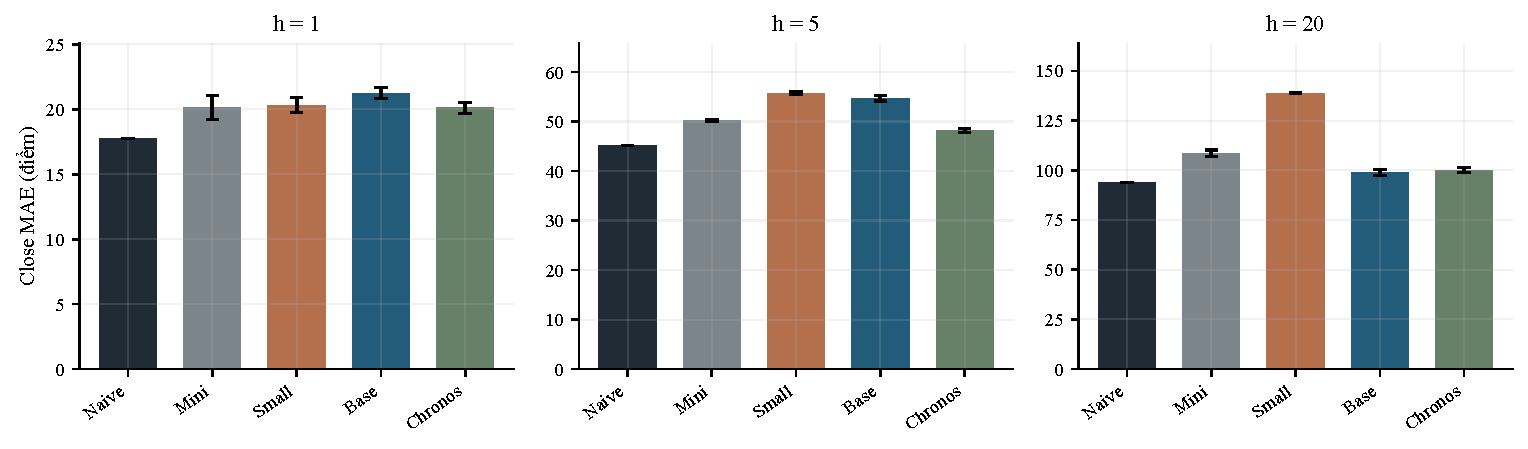
\includegraphics[width=\linewidth]{main_close.pdf}
\caption{Close MAE của Naive và bốn neural model SFT. Error bar là SD
giữa seed, không phải confidence interval.}
\label{fig:main}
\end{figure}

Trong các Kronos SFT, base có Close $h=20$ MAE thấp nhất ở \BaseSFT{}
điểm; mini đạt \MiniSFT{} và small đạt \SmallSFT{}. Ở $h=1/5$, mini
có mean MAE thấp hơn small và base. Chronos best-trained SFT đạt
\ChronosSFT{} điểm tại $h=20$. Các kết quả này cho thấy thứ hạng phụ
thuộc horizon; chưa có ưu thế tổng thể của neural model trước Naive
trong protocol đã thử.

\subsection{Open và đặc điểm của label}\label{sec:open}
Open h=1 MAE của Naive là 5,959 điểm, thấp hơn các neural model.
Một phần kết quả liên quan tới cấu trúc label: trong 323 test origins,
có 59 origins mà target thuộc đoạn Open bằng Close trước. Vì Naive
predict bằng Close tại origin, error trên nhóm này bằng 0; trên 264
origins còn lại, Open MAE của Naive là 7,291.

Ví dụ dữ liệu thật: Close ngày 20/05/2025 là 1.407,52; Open ngày
21/05/2025 cũng bằng 1.407,52; Naive predict Open là 1.407,52,
nên absolute error bằng 0. Không có rule riêng cho nhóm 59 origins và
không sử dụng target tương lai. Do đó, Open MAE cần được đọc cùng định
nghĩa và cách dựng nhãn của nguồn, chưa thể đồng nhất với khả năng
predict giá mở cửa chính thức. Bảng Open đầy đủ ở Phụ lục~\ref{app:open}.
\FloatBarrier

\subsection{Q2: Model size và tác động SFT}
SFT tạo cải thiện rõ cho Kronos-base ở horizon dài:
Close $h=20$ MAE giảm \BaseGain{} điểm, từ \BaseZero{} xuống
\BaseSFT{}, tương đương \BaseGainPct\% so với zero-shot
(Hình~\ref{fig:size}). Mini và small cũng giảm Close $h=20$ MAE sau SFT,
nhưng mức cải thiện không đồng đều ở các horizon. Riêng base tại $h=1$,
MAE tăng nhẹ từ 20,889 lên 21,234, nên không diễn giải SFT như cải thiện
mọi target và horizon.

\begin{figure}[htbp]
\centering
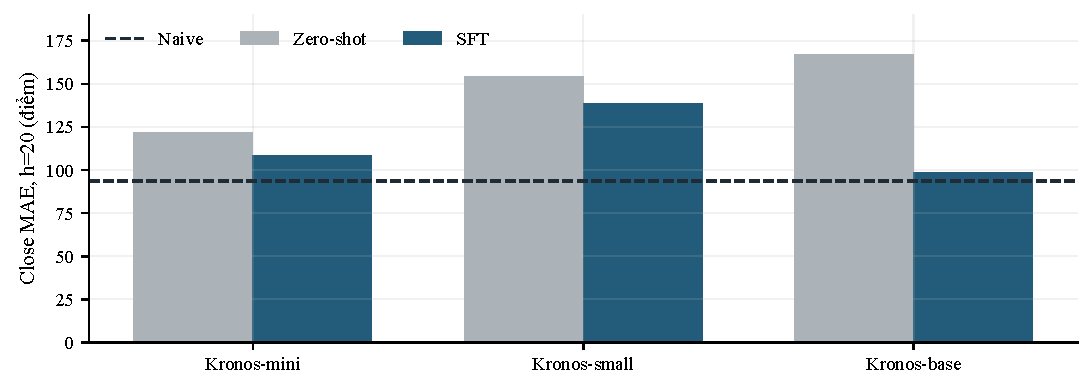
\includegraphics[width=.9\linewidth]{size_sft.pdf}
\caption{Zero-shot và best-trained SFT của ba Kronos tại Close $h=20$.
Đường đứt là Naive, giúp đặt mức cải thiện SFT trong cùng thang so sánh.}
\label{fig:size}
\end{figure}

Mini SFT có MAE thấp hơn small SFT ở cả ba horizon, đồng thời có chi phí
thấp hơn. Sự khác biệt tokenizer ngăn việc quy toàn bộ khác biệt này
cho số tham số. Bảng~\ref{tab:cost} bổ sung chi phí của từng hệ thống.

\begin{table}[htbp]
\centering\small
\caption{Chi phí SFT, mean ba seed trên RTX 4070 SUPER 12 GB.}
\label{tab:cost}
\begin{tabular}{@{}lrrr@{}}
\toprule
Model & Tham số (M) & SFT 5 epoch/seed (s) & Peak tensor (GiB) \\
\midrule
Kronos-mini & 4,1 & 20,5 & 0,198 \\
Kronos-small & 24,7 & 36,9 & 0,780 \\
Kronos-base & 102,3 & 87,4 & 2,543 \\
Chronos-2-small & 27,9 & 48,2 & 0,564 \\
\bottomrule
\end{tabular}

\end{table}

Thời gian trong bảng là \textbf{giai đoạn SFT năm epoch của một seed},
lấy mean qua ba seed. Timer bắt đầu sau setup model và, với Kronos,
sau encode dữ liệu bằng tokenizer cố định; gồm initial validation,
train, validation và lưu checkpoint, không gồm download/load/tokenize
hay toàn bộ inference pipeline. Peak tensor memory là lượng bộ nhớ do
PyTorch ghi nhận, khác tổng VRAM process. Thời gian ngắn phản ánh
data budget nhỏ và teacher forcing, không chứng minh train đã đủ.

\subsection{Q2: Quantize ablation}
Ablation sử dụng cùng encoder tokenizer small cố định, cùng random
small backbone, numeric head/MSE, data và train budget. Nhánh continuous
dùng features L2-normalized trước BSQ; nhánh quantized dùng features sau
BSQ. Initialization của predictor được ghép cặp theo seed.

\begin{table}[htbp]
\centering\small
\caption{Quantize ablation: Close MAE, mean $\pm$ SD ba seed.}
\label{tab:ablation}
\begin{tabular}{@{}lrrr@{}}
\toprule
Representation & $h=1$ & $h=5$ & $h=20$ \\
\midrule
Continuous & 22,832 $\pm$ 1,255 & 66,015 $\pm$ 9,060 & 144,375 $\pm$ 16,360 \\
Quantized & 22,832 $\pm$ 0,134 & 67,571 $\pm$ 4,365 & 150,927 $\pm$ 5,131 \\
\bottomrule
\end{tabular}

\end{table}

\begin{figure}[htbp]
\centering
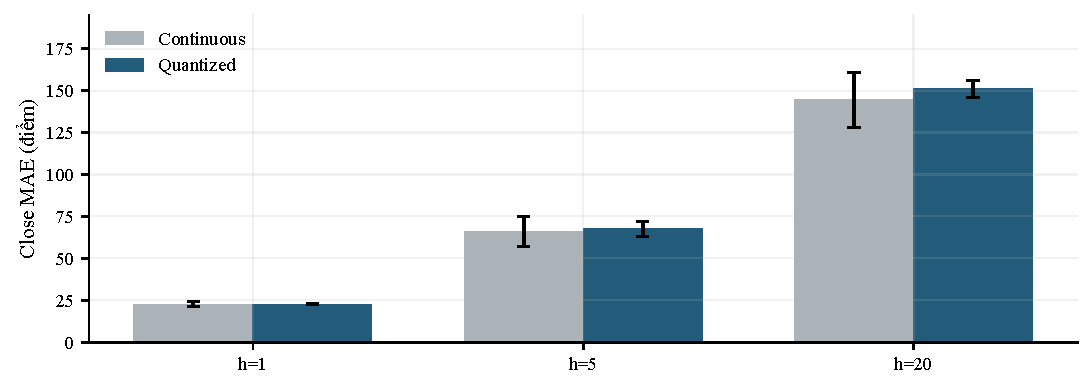
\includegraphics[width=.9\linewidth]{ablation.pdf}
\caption{So representation trước/sau quantize trong ablation cố định.
Error bar là SD giữa seed.}
\label{fig:ablation}
\end{figure}

Hai nhánh gần bằng nhau tại $h=1$. Quantized có MAE mean cao hơn tại
$h=5/20$, trong khi SD giữa seed ở một số ô khá lớn. Chưa có bằng chứng
quantize giúp Close MAE giảm đồng nhất trong ablation này. Kết luận chỉ
áp dụng cho bước can thiệp đã thiết kế, không đánh giá riêng mọi thành
phần của K-line representation hay toàn bộ hệ thống pre-trained.
\FloatBarrier

\subsection{Q3: Data budget và predictor pre-training}
Kronos-small và Chronos-2-small được chọn cho learning curve với
500 / 1.000 / 1.589 session train, tương ứng 353 / 853 / 1.442 windows.
Các đoạn train lồng nhau, cùng ngày kết thúc, giữ validation/test cố định.
Pre-trained được so với predictor cùng kiến trúc khởi tạo ngẫu nhiên.
Random Kronos vẫn sử dụng tokenizer pre-trained.

Mỗi trial tối đa năm epoch. Pre-trained giữ learning rate chính
$10^{-6}$; random chọn learning rate từ $\{10^{-6},10^{-5},10^{-4}\}$
bằng validation. Vì vậy, tổng search cost không bằng nhau dù budget
của từng trial giống nhau. Hình~\ref{fig:learning} trình bày Close $h=20$;
ba horizon đầy đủ ở Phụ lục~\ref{app:learning}.

\begin{figure}[htbp]
\centering
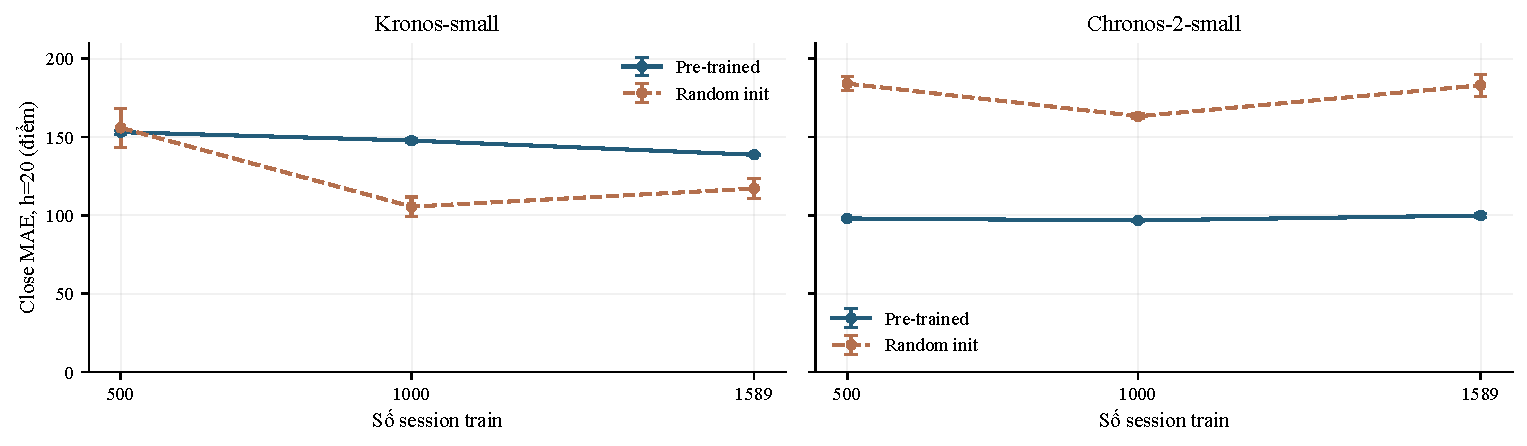
\includegraphics[width=\linewidth]{learning.pdf}
\caption{Learning curve tại Close $h=20$. Error bar là SD ba seed.
Pre-trained chỉ predictor bắt đầu từ weight đã học; random chỉ random
initialization của predictor trong thiết lập tương ứng.}
\label{fig:learning}
\end{figure}

Chronos pre-trained có MAE thấp hơn random trong cả chín ô
budget/horizon. Với Kronos-small, lợi ích không đồng nhất: tại
1.000 session, random tốt hơn pre-trained ở $h=5/20$; full budget cũng
có kết quả tương tự ở hai horizon này. Riêng Close $h=20$ full,
random đạt 117,220 so với pre-trained \SmallSFT{} điểm.
Trong nhánh Kronos pre-trained, thêm data cải thiện $h=20$ nhưng không
làm mọi horizon cùng tốt hơn. Các kết luận giới hạn trong search space
và training budget đã thử.
\FloatBarrier

\subsection{Q4: Seed, horizon và khoảng bất định}
Để giữ cấu trúc phụ thuộc của các forecast origins chồng lấn,
paired moving-block bootstrap được áp dụng cho chênh lệch absolute
error với Naive, cùng origins, block dài 20 và 2.000 lần lấy mẫu
\citep{kunsch1989bootstrap}. CI percentile 95\% dùng RNG seed 42.
SD giữa ba training seed và bootstrap CI trả lời hai câu hỏi khác nhau;
không ghép ba seed thành các thị trường độc lập.

\begin{figure}[htbp]
\centering
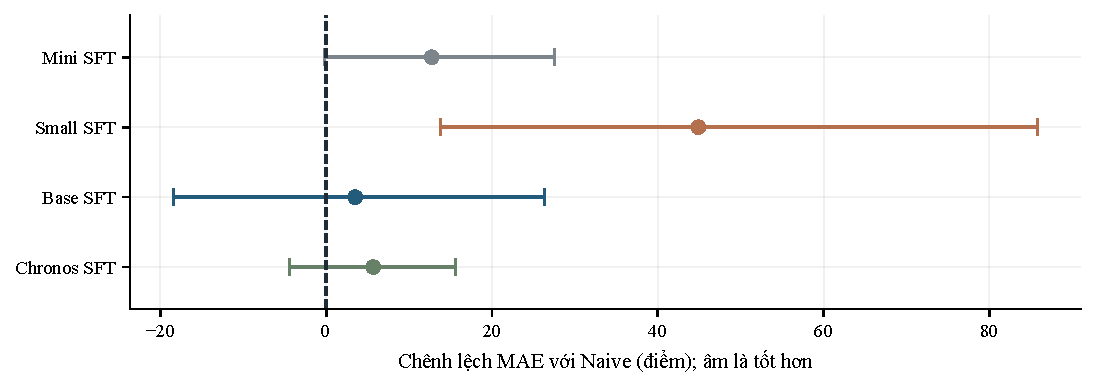
\includegraphics[width=.9\linewidth]{intervals_h20.pdf}
\caption{Chênh lệch Close $h=20$ MAE với Naive, neural seed 42 và CI 95\%.
Âm nghĩa là tốt hơn Naive; CI cắt 0 chưa cho thấy khác biệt rõ trong
phép kiểm này. Bảng ba horizon ở Phụ lục~\ref{app:ci}.}
\label{fig:ci}
\end{figure}

Base SFT có chênh lệch $3,488$ điểm tại $h=20$, CI
$[-18,439;\,26,387]$, còn small SFT có chênh lệch $44,896$ điểm với CI
$[13,737;\,85,757]$. CI chưa điều chỉnh multiple comparisons và còn phụ
thuộc lựa chọn block. Các khoảng này giúp phân biệt chênh lệch số học
với mức bất định, không chứng minh hai model tương đương khi cắt 0.

\subsection{Q4: Giai đoạn và volatility}
Volatility tại origin $t$ là SD của 20 log-return đã quan sát:
\begin{equation}
 r_t=\log(C_t/C_{t-1}),\qquad
 v_t=\mathrm{SD}(r_{t-19},\ldots,r_t),\quad \mathrm{ddof}=1.
\end{equation}
Threshold p90 chỉ lấy từ train và giữ cố định cho test. Test có
17/323 origins vượt threshold, tạo hai cụm: 6 origins từ 11--18/03/2026
và 11 origins từ 20/03--03/04/2026. Rolling windows chồng lấn nên các
origin trong một cụm không đại diện các biến cố độc lập.

\begin{table}[htbp]
\centering\small
\caption{Close $h=20$ MAE theo ba đoạn test và nhóm volatility cao,
mean ba seed. Ba đoạn có 108/108/107 origins; high-volatility có 17 origins.}
\label{tab:regime}
\begin{tabular}{@{}lrrrr@{}}
\toprule
Model & Đoạn 1 & Đoạn 2 & Đoạn 3 & High-vol. \\
\midrule
Naive & 109,977 & 98,685 & 72,618 & 159,355 \\
Mini SFT & 153,116 & 92,096 & 79,993 & 141,836 \\
Small SFT & 236,885 & 96,716 & 82,023 & 127,385 \\
Base SFT & 108,828 & 102,620 & 84,971 & 112,710 \\
Chronos SFT & 103,874 & 111,084 & 84,830 & 188,250 \\
\bottomrule
\end{tabular}

\end{table}

Base SFT có kết quả tốt hơn Naive trong đoạn 1 và nhóm high-volatility
ở metric này, nhưng không giữ lợi thế ở mọi đoạn. Chronos SFT và
Kronos-small SFT cũng có thứ hạng thay đổi theo giai đoạn. Do coverage
của nhóm volatility cao còn ít, bảng được dùng để mô tả tính phụ thuộc
điều kiện, chưa khẳng định độ bền qua nhiều đợt khủng hoảng.

\subsection{Q4: Hai expanding-window fold}
Mỗi fold gồm train/validation/test theo thời gian, với train mở rộng ở
fold sau. Fold 1 kết thúc train ngày 11/03/2022, validation
14/03/2022--08/02/2023, test 09/02--29/12/2023. Fold 2 kết thúc train
ngày 08/02/2023, validation 09/02--29/12/2023, test
02/01--28/11/2024. Mỗi fold có 208 test origins, neural seed 42,
chọn checkpoint bằng validation riêng.

Chronos SFT nhỉnh hơn Naive tại fold 1 $h=5$ (22,213 so với 22,363),
nhưng không giữ lợi thế ở fold 2. Nhìn chung, chưa có neural model
thắng nhất quán cả ba horizon và hai fold
(Phụ lục~\ref{app:fold}). Cả hai fold có 0 origins high-volatility theo
threshold train riêng, nên chúng bổ sung kiểm tra theo thời gian nhưng
chưa bổ sung bằng chứng về nhóm volatility cao.
\FloatBarrier

\section{Thảo luận}
Kết quả cho thấy SFT có thể điều chỉnh một model pre-trained để phù hợp
hơn với horizon của bài toán. Mức giảm MAE của base ở $h=20$ là ví dụ
rõ, đồng thời bảng toàn bộ horizon cho thấy cải thiện này không phổ quát.
Mini mang lại cân bằng đáng chú ý giữa chi phí và error, còn baseline
Naive giữ vai trò tham chiếu cần thiết khi predict mức giá chỉ số.
Một MAE thấp cần được đặt trong cùng target, origins và cấu trúc label.

Ba điểm giới hạn cần giữ khi diễn giải là: nhãn OHLC còn khác biệt
giữa nguồn; evaluation mang tính hồi cứu và chưa xác minh đầy đủ
pre-training cutoff của từng revision; năm epoch và một số ít giai đoạn
không đại diện tối ưu đến hội tụ hay mọi trạng thái thị trường.
Đặc biệt, test lịch sử đã từng được xem trong nghiên cứu trước, nên
không mô tả đây là một triển khai lịch sử hoàn toàn mới.
Việc đánh giá tập trung vào MAE/RMSE mức giá, không suy trực tiếp
thành lợi nhuận giao dịch hoặc kết quả sau chi phí.

\section{Kết luận}
Nghiên cứu cung cấp một đánh giá thống nhất cho Kronos mini/small/base,
Chronos-2-small và bốn baseline trên VN30. Đối với Q1, neural model chưa
thể hiện lợi thế ổn định trước Naive trong bảng chính. Đối với Q2, SFT
cải thiện rõ base ở Close $h=20$, trong khi model size và quantize chưa
cho lợi ích đồng nhất. Đối với Q3, tác dụng predictor pre-training phụ
thuộc model và data budget; thêm data chưa giúp mọi horizon. Đối với Q4,
error và thứ hạng thay đổi theo thời gian, horizon và mức volatility.

Giá trị của kết quả nằm ở việc xác định điều kiện mà mỗi hệ thống hoạt
động tốt hơn, cùng một protocol minh bạch để so sánh và tái lập, thay
vì chỉ lựa chọn một model theo kích thước hoặc một điểm số đơn lẻ.
Các bảng, code và phiên bản dữ liệu thực nghiệm được lưu trong kho
dự án \citep{vn30repository}.

\begingroup
\small
\setlength{\bibsep}{3pt}
\bibliographystyle{plainnat}
\bibliography{references}
\endgroup
\clearpage
\appendix
\section{Bảng kết quả bổ sung}
\subsection{Open MAE}\label{app:open}
\begin{table}[htbp]
\centering\small
\caption{Open MAE trên test, mean $\pm$ SD ba seed; quy ước như Bảng~\ref{tab:close}.}
\begin{tabular}{@{}lrrr@{}}
\toprule
Model & $h=1$ & $h=5$ & $h=20$ \\
\midrule
Naive & \textbf{5,959} & \textbf{40,846} & \textbf{91,951} \\
Ridge & 12,392 & 45,368 & 103,683 \\
ARIMA & 18,999 & 46,270 & 94,720 \\
ETS & 19,017 & 46,288 & 94,700 \\
\midrule
Kronos-mini & 9,726 $\pm$ 0,111 & 49,886 $\pm$ 1,208 & 120,706 $\pm$ 0,866 \\
Kronos-mini SFT & 9,806 $\pm$ 0,100 & 46,878 $\pm$ 0,527 & 107,852 $\pm$ 1,582 \\
Kronos-small & 10,428 $\pm$ 0,206 & 48,808 $\pm$ 0,618 & 151,298 $\pm$ 1,071 \\
Kronos-small SFT & 10,208 $\pm$ 0,262 & 52,177 $\pm$ 0,445 & 131,519 $\pm$ 1,763 \\
Kronos-base & 10,408 $\pm$ 0,178 & 50,477 $\pm$ 0,377 & 164,544 $\pm$ 0,439 \\
Kronos-base SFT & 10,466 $\pm$ 0,313 & 49,770 $\pm$ 0,714 & 97,545 $\pm$ 1,373 \\
Chronos-2-small & 21,045 & 48,651 & 103,229 \\
Chronos-2-small SFT & 20,671 $\pm$ 0,555 & 48,740 $\pm$ 0,518 & 100,810 $\pm$ 1,251 \\
\bottomrule
\end{tabular}

\end{table}

\subsection{Learning curve tại ba horizon}\label{app:learning}
\begin{table}[htbp]
\centering\small
\caption{Close MAE theo data budget và initialization, mean ba seed.
Full budget là 1.589 session.}
\begin{tabular}{@{}lrrrrr@{}}
\toprule
Model & Init. & Session & $h=1$ & $h=5$ & $h=20$ \\
\midrule
Kronos-small & Pre-trained & 500 & 20,067 & 50,523 & 153,161 \\
Kronos-small & Pre-trained & 1.000 & 20,325 & 53,489 & 147,780 \\
Kronos-small & Pre-trained & 1.589 & 20,326 & 55,690 & 138,716 \\
Kronos-small & Random & 500 & 32,188 & 86,797 & 155,908 \\
Kronos-small & Random & 1.000 & 21,925 & 52,265 & 105,597 \\
Kronos-small & Random & 1.589 & 21,743 & 54,729 & 117,220 \\
\midrule
Chronos-2-small & Pre-trained & 500 & 19,753 & 47,364 & 98,074 \\
Chronos-2-small & Pre-trained & 1.000 & 19,498 & 47,449 & 96,782 \\
Chronos-2-small & Pre-trained & 1.589 & 20,104 & 48,198 & 99,976 \\
Chronos-2-small & Random & 500 & 152,647 & 160,078 & 184,120 \\
Chronos-2-small & Random & 1.000 & 129,054 & 140,272 & 163,259 \\
Chronos-2-small & Random & 1.589 & 149,456 & 157,607 & 183,093 \\
\bottomrule
\end{tabular}

\end{table}
\FloatBarrier
\clearpage

\subsection{Paired bootstrap intervals}\label{app:ci}
\begin{table}[htbp]
\centering\small
\caption{Chênh lệch Close MAE với Naive và CI 95\%, seed 42, $n=323$.
Block 20 origins, 2.000 lần lấy mẫu.}
\begin{tabular}{@{}lrrr@{}}
\toprule
Model & $h$ & $\Delta$MAE & CI 95\% \\
\midrule
Mini SFT & 1 & 1,657 & [0,369; 2,820] \\
Mini SFT & 5 & 4,779 & [1,732; 8,373] \\
Mini SFT & 20 & 12,738 & [-0,257; 27,575] \\
Small SFT & 1 & 1,923 & [-0,435; 4,147] \\
Small SFT & 5 & 10,443 & [1,700; 22,576] \\
Small SFT & 20 & 44,896 & [13,737; 85,757] \\
Base SFT & 1 & 3,031 & [0,899; 5,149] \\
Base SFT & 5 & 9,236 & [1,284; 17,878] \\
Base SFT & 20 & 3,488 & [-18,439; 26,387] \\
Chronos SFT & 1 & 1,935 & [0,734; 3,010] \\
Chronos SFT & 5 & 2,772 & [-0,539; 5,990] \\
Chronos SFT & 20 & 5,666 & [-4,396; 15,555] \\
\bottomrule
\end{tabular}

\end{table}
\FloatBarrier

\subsection{Kết quả hai fold}\label{app:fold}
\begin{table}[htbp]
\centering\small
\caption{Close MAE trên hai fold, neural seed 42, 208 origins/fold.
SFT dùng best-trained; mỗi fold có train/validation riêng.}
\begin{tabular}{@{}lrrrr@{}}
\toprule
Fold & Model & $h=1$ & $h=5$ & $h=20$ \\
\midrule
1 & Naive & 9,472 & 22,363 & 40,009 \\
1 & Kronos-mini & 10,541 & 25,600 & 50,098 \\
1 & Kronos-mini SFT & 10,474 & 23,655 & 49,682 \\
1 & Kronos-small & 11,039 & 27,526 & 57,831 \\
1 & Kronos-small SFT & 10,990 & 27,708 & 59,611 \\
1 & Kronos-base & 10,683 & 26,395 & 66,885 \\
1 & Kronos-base SFT & 11,524 & 25,392 & 56,358 \\
1 & Chronos-2-small & 10,829 & 24,046 & 44,165 \\
1 & Chronos-2-small SFT & 10,417 & 22,213 & 40,958 \\
\midrule
2 & Naive & 8,395 & 20,580 & 36,072 \\
2 & Kronos-mini & 9,592 & 22,950 & 45,265 \\
2 & Kronos-mini SFT & 9,779 & 22,362 & 41,484 \\
2 & Kronos-small & 9,515 & 21,456 & 43,456 \\
2 & Kronos-small SFT & 10,216 & 24,614 & 40,315 \\
2 & Kronos-base & 9,965 & 21,526 & 53,029 \\
2 & Kronos-base SFT & 10,087 & 26,404 & 42,151 \\
2 & Chronos-2-small & 9,241 & 21,020 & 37,369 \\
2 & Chronos-2-small SFT & 10,449 & 21,978 & 42,643 \\
\bottomrule
\end{tabular}

\end{table}
\FloatBarrier

\subsection{Phiên bản và khả năng tái lập}
Dataset SHA256:
\begin{quote}\footnotesize\ttfamily
\path{fee0bd8c240a9d2be4ef5c9d287eede6c5506b0358c25545e72de99709da4fd2}
\end{quote}
Manifest lưu revision model/tokenizer, split, seed, aggregation và
checkpoint selection. Bảng/hình sinh từ CSV đã kiểm tra, không train
hay inference lại. Snapshot giữ hàng ngoài request ở 01/10/2026 và
không bổ sung dữ liệu trước 2017.

\end{document}
